% ============================================================
% EqWM-FPS: Equivariant World Models for Sample-Efficient
% Imagination Training in a First-Person Shooter
% Submitted to: Neural Networks (Elsevier)
%
% To switch to ECAI/UAI: change the \documentclass line and the
% \journalnote below; body content is unchanged.
% ============================================================
\documentclass[preprint,12pt]{elsarticle}
% ECAI/UAI switch: replace the line above with, e.g.,
%   \documentclass[10pt,a4paper]{article}
% and use natbib/icml style; the body is journal-agnostic.

\journal{Neural Networks}

\usepackage{graphicx}
\usepackage{amsmath,amssymb}
\usepackage{booktabs}
\usepackage{multirow}
\usepackage{xcolor}
\usepackage{url}
\usepackage{enumitem}
\graphicspath{{figs/}}

% theorem-like environments
\newtheorem{theorem}{Theorem}
\newtheorem{proposition}{Proposition}

\bibliographystyle{elsarticle-num}

\begin{document}

\begin{frontmatter}

\title{Equivariant World Models for Sample-Efficient Imagination\\
Training in a First-Person Shooter: An Empirical Study}

\author[1]{Anonymous}
\address[1]{Anonymous Institution (double-blind review)}

\begin{abstract}
First-person shooter (FPS) games are a stress test for deep reinforcement
learning (RL): visual observations are high-dimensional and sample
complexity is prohibitive. World models and imagination training
\cite{worldmodels2018,dreamerv3} reduce real-environment interaction by
training a policy inside a learned dynamics model, but most implementations
ignore a structural symmetry that FPS environments possess almost by
construction: left--right mirror symmetry. We study \emph{EqWM}, a compact
world model and PPO policy that enforce horizontal-flip ($\mathbb Z_2$)
equivariance by group averaging across the encoder, recurrent dynamics,
decoder, and reward head, evaluated on the ViZDoom \texttt{health\_gathering}
benchmark \cite{vizdoom2016}. We also derive PAC-Bayes-style bounds that
decompose the imagination-training risk into world-model bias and
statistical-estimation terms, and a scaling law for the optimal
real-to-imagination ratio. Our empirical findings are deliberately reported
without inflation. (i)~With only $10$k environment steps and three seeds, the
equivariant world model has a substantially more stable reward head: reward
prediction MAE is $0.104\pm0.025$ versus $0.223\pm0.099$ for a
non-equivariant baseline, where the higher baseline mean is driven by
seed-to-seed divergence (two of three baseline seeds drift to
$0.26$--$0.32$ rather than uniformly worse accuracy); single-frame
reconstruction (PSNR/SSIM) is statistically indistinguishable and in fact
marginally favors the non-equivariant model. (ii)~Imagination training
reaches, after only $\sim$15k real steps, episode returns comparable to pure
on-policy PPO at $20$k--$40$k real steps, i.e. an order-of-$2\times$
sample-efficiency gain (the measured step ratio is $\sim$1.3--2.7$\times$;
because both curves are flat and noisy this is an order-of-magnitude
comparison, not a clean crossover); under this small-model budget the
equivariant and non-equivariant imagination variants win on different seeds
and are not statistically distinguishable. (iii)~A four-cell ablation
(whether equivariance lives in the world model, the policy, both, or
neither) yields final returns of $447\pm38$, $425\pm29$, $427\pm27$, and
$450\pm47$ that overlap inside their error bars: at this budget no
equivariant component produces a significant return gain. (iv)~A bootstrap
estimate of the effective-sample multiplier is non-monotone in training
length and inconsistent across two machines, so we report any multiplier
above $1$ as an open problem rather than a confirmed result. We
present the theory as an upper bound and a scaling law, and we explicitly
mark where experiments support, weakly support, or contradict it.
\end{abstract}

\begin{keyword}
Equivariant neural networks \sep World models \sep Imagination training \sep Reinforcement learning \sep First-person shooter \sep PAC-Bayes
\end{keyword}

\end{frontmatter}

%% ===================== 1. INTRODUCTION =====================
\section{Introduction}
Deep reinforcement learning (RL) has reached superhuman levels in many
games, but training an agent directly from raw pixels in first-person
shooters (FPS) still demands millions of environment interactions
\cite{fps2017,vizdoom2016}, which is impractical when environment access is
expensive. \emph{World models} address this by learning a predictive model
of the environment and optimizing the policy entirely inside it
\cite{worldmodels2018}. The Dreamer family operationalizes this idea with a
recurrent state-space model \cite{dreamerv1,dreamerv2,dreamerv3} and has
recently scaled to long-horizon tasks inside learned models
\cite{dreamer42025}; model-based planning with a learned dynamics model is
the core of MuZero \cite{muzero2020}, and model-based policy optimization
exploits such models for data efficiency \cite{mbpo2019}.

FPS environments, however, possess a near-perfect structural symmetry that
none of these general-purpose architectures exploit: the rendered scene and
its dynamics are (approximately) invariant under a horizontal flip, and a
flipped camera view should induce flipped actions
(TURN\_LEFT $\leftrightarrow$ TURN\_RIGHT, MOVE\_FORWARD unchanged).
Group-equivariant networks \cite{gcnn2016} bake such symmetries into the
architecture and, in principle, use each observation several times at no extra
data cost. This is precisely the data-starved regime in which world models
operate.

We ask a deliberately narrow question: \emph{on a small FPS benchmark, does
$\mathbb Z_2$ equivariance in the world model and policy improve sample
efficiency, and how should that be measured honestly?} Our system,
\emph{EqWM}, enforces hard equivariance by group averaging
\cite{gcnn2016} at every convolutional layer of the encoder, recurrent
dynamics, decoder, and policy, with an invariant reward head and an
antisymmetric left/right action head. Our contributions are:
\begin{enumerate}[leftmargin=*]
  \item \textbf{Implementation and controlled comparison on ViZDoom.} We
        build an equivariant ConvGRU world model and equivariant PPO policy
        for \texttt{health\_gathering} and compare them against matched
        non-equivariant baselines, reporting per-seed as well as aggregated
        numbers (Section~\ref{sec:exp}).
  \item \textbf{PAC-Bayes-style analysis of imagination training.} We state
        three results: a world-model prediction bound that depends on an
        effective sample count $N_{\rm eff}$ (Theorem~\ref{th:wm}), an
        imagination-training generalization bound that separates world-model
        bias from estimation error (Theorem~\ref{th:imag}), and a scaling law
        for the optimal real-to-imagination ratio (Theorem~\ref{th:ratio});
        proof sketches and a bootstrap estimator (Proposition~\ref{prop:meff})
        are provided.
  \item \textbf{Honest empirical verdict.} The clearest measured benefit of
        equivariance is \emph{cross-seed stability of the task-relevant
        reward head}, not a large mean accuracy gain; imagination training
        gives an order-of-$2\times$ sample-efficiency gain over pure
        PPO; the ablation shows no significant return gain from equivariance
        at this budget; and the bootstrap estimate of the multiplier is not
        robust. We treat the latter two as limitations and open problems
        rather than burying them.
\end{enumerate}

The remainder of the paper is organized as follows. Section~\ref{sec:rw}
reviews related work. Section~\ref{sec:prelim} fixes notation.
Section~\ref{sec:method} details the architecture. Section~\ref{sec:theory}
states the theory. Section~\ref{sec:exp} reports experiments, and
Section~\ref{sec:concl} concludes with limitations.

%% ===================== 2. RELATED WORK =====================
\section{Related Work}\label{sec:rw}

\paragraph{World models and imagination training.}
Learning a predictive model for RL dates back to Ha and Schmidhuber
\cite{worldmodels2018}. The Dreamer series \cite{dreamerv1,dreamerv2}
operationalized latent imagination with a recurrent state-space model, and
DreamerV3 \cite{dreamerv3} showed a single model can solve many domains; the
most recent Dreamer4 \cite{dreamer42025} scales agent training inside a
fast world model in Minecraft. MuZero \cite{muzero2020} pairs learned
dynamics with planning, and MBPO \cite{mbpo2019} uses an ensemble of models
to cut real samples. Concurrent with these, EMERALD \cite{emerald2025}
improves world modeling with masked latent transformers and strong
sample efficiency on Crafter. Our work follows the Dreamer-style
``train PPO inside a learned latent model'' loop but restricts the model class
to a group-equivariant one.

\paragraph{Equivariant reinforcement learning.}
Group-equivariant convolutions were introduced by Cohen and Welling
\cite{gcnn2016}. In RL, MDP homomorphic networks \cite{mdphomo2020} and group
equivariant deep RL \cite{geodrl2020} encode state/action symmetries, while
$\mathrm{SO}(2)$-equivariant policies \cite{so2rl2022} and group-invariant
representation structuring \cite{groupinv2022} exploit continuous rotation
symmetries. The closest lines to ours are equivariant model-based RL: Park
et al.\ learn symmetric embeddings for equivariant world models
\cite{sen2022}, Deac et al.\ make MuZero equivariant \cite{eqmuzero2023},
and EDGI builds an SE(3)-equivariant diffusion planner for embodied agents
\cite{edgi2023}. Multi-group equivariant augmentation \cite{multigroup2025}
studies several symmetry groups in manipulation. Unlike these works, which
target control, board games, or 3D/SE(3) embodied settings, we target 2D
FPS pixels with the discrete $\mathbb Z_2$ group and integrate equivariance
into \emph{both} the world model and the imagination-training loop, while
reporting the small-benchmark result transparently.

\paragraph{PAC-Bayes and generalization in RL.}
PAC-Bayes bounds \cite{mcallester1999} relate a posterior's risk to its
empirical risk through a KL complexity term. Recent PAC-Bayesian RL
\cite{pacbayesrl2025} trains generalizable on-policy policies. We adapt the
decomposition to the mixed real/imagination data regime and use the bootstrap
\cite{bootstrap1993} to estimate the effective sample multiplier empirically.

\paragraph{FPS reinforcement learning.}
ViZDoom \cite{vizdoom2016} provides a Doom-based visual-RL benchmark; early
agents trained directly with model-free RL \cite{fps2017}. To our knowledge,
prior work has not combined an equivariant world model with imagination
training on FPS pixels.

%% ===================== 3. PRELIMINARIES =====================
\section{Preliminaries}\label{sec:prelim}

\paragraph{MDP.}
We model the environment as an MDP
$\langle\mathcal S,\mathcal A,P,r,\gamma\rangle$ \cite{suttonbarto2018},
where $\mathcal S$ is the RGB frame space,
$\mathcal A=\{\textsc{turn-left},\textsc{turn-right},\textsc{forward}\}$ is a
three-action discrete set, $P$ the transition kernel, $r$ the reward, and
$\gamma=0.99$ the discount. The objective is the expected discounted return
$J(\pi)=\mathbb E_{\pi}[\sum_t\gamma^t r_t]$.

\paragraph{Group action and equivariance.}
We take $G=\mathbb Z_2=\{e,h\}$, where $h$ is a horizontal flip. The group
acts on observations by $h\cdot x=\mathrm{flip}_W(x)$ and on actions by the
permutation $h\cdot\textsc{turn-left}=\textsc{turn-right}$,
$h\cdot\textsc{turn-right}=\textsc{turn-left}$,
$h\cdot\textsc{forward}=\textsc{forward}$. A map $f$ is
\emph{equivariant} if $f(gx)=g f(x)$ and \emph{invariant} if $f(gx)=f(x)$.

\paragraph{World models and imagination.}
A world model $\hat M=\langle\hat P,\hat r\rangle$ approximates the
environment. Given $\hat M$, imagination training starts a policy rollout
from a real observation and predicts subsequent latent states and rewards
with $\hat M$, then updates the policy (here PPO \cite{ppo2017}) on these
imagined trajectories \cite{dreamerv3}.

\paragraph{PAC-Bayes.}
With posterior $\rho$, prior $\pi$, and $n$ i.i.d.\ samples, a canonical
bound is
$R(\rho)\le R_S(\rho)+\sqrt{(\mathrm{KL}(\rho\|\pi)+\log(2\sqrt n/\delta))/(2n)}$.

%% ===================== 4. METHOD =====================
\section{Method}\label{sec:method}

\subsection{Equivariant $\mathbb Z_2$ world model}
The world model $\hat M_\phi$ has four parts.
\emph{Encoder} $E_\phi$: three strided convolutions map a
$64\times64\times3$ frame to an $8\times8\times z$ latent map
($z=32$, base channels $16$). Every convolution is a group-averaging layer
\cite{gcnn2016},
\begin{equation}
  E_\phi(x)=\tfrac12\big[\mathrm{Conv}(x)+\mathrm{flip}_W(\mathrm{Conv}(\mathrm{flip}_W(x)))\big],
\end{equation}
which shares one kernel and satisfies
$E_\phi(\mathrm{flip}_W x)=\mathrm{flip}_W E_\phi(x)$ up to numerical
precision. \emph{Dynamics}: an equivariant ConvGRU cell updates the latent
map from the previous map and a spatially broadcast one-hot action; gates
use the same group-averaging convolution. \emph{Decoder}: three equivariant
transposed convolutions reconstruct the frame with a sigmoid output.
\emph{Reward head}: a global-average-pooling (invariant) layer followed by an
MLP predicts a scalar reward from the latent map. The non-equivariant
baseline uses identical widths and layer counts but ordinary convolutions, a
flattened encoder for its heads, and no group averaging.

The training loss is reconstruction MSE plus reward MSE plus latent-dynamics
MSE, and (only for the equivariant model) a soft consistency penalty on the
encoder and dynamics under flip.

\subsection{Equivariant PPO policy}
The policy uses the same equivariant encoder. Invariant features
($\mathrm{gap}(h)$) drive the forward action and the (invariant) value head;
an antisymmetric feature $a=\overline{h_{\rm left}}-\overline{h_{\rm right}}$
distinguishes left and right:
$\ell_{\rm left}=s+a$, $\ell_{\rm right}=s-a$, $\ell_{\rm forward}=s'$.
This enforces $\pi(h\cdot x)=h\cdot\pi(x)$.

\subsection{Imagination pipeline}
We collect $n=10$k random real transitions, train $\hat M_\phi$ for 30
epochs, then iterate: collect $1{,}000$ new on-policy real transitions,
fine-tune $\hat M_\phi$ for 5 epochs, imagine short rollouts of horizon
$H=20$ under PPO \cite{ppo2017} (200 rollouts per outer step), and update on
the imagined data. This gives roughly $4{,}000$ imagined transitions per
$1{,}000$ new real transitions, i.e.\ an imagination ratio $\approx4$, fixed
rather than tuned. Table~\ref{tab:hyper} lists all hyper-parameters.

\begin{table}[t]
\centering
\caption{Hyper-parameters (identical for equivariant and standard variants
except for group averaging). Exp.\,1 trained the world model for 50 epochs;
the imagination runs below use 30 initial epochs.}
\label{tab:hyper}
\begin{tabular}{lll}
\toprule
Group & Hyper-parameter & Value \\
\midrule
Environment & Observation & $64\times64\times3$ RGB, frame skip $4$ \\
            & Discount $\gamma$ & $0.99$ \\
World model & Base channels / latent $z$ & $16$ / $32$ ($8\times8\times32$) \\
            & Init. real steps $n$ & $10{,}000$ \\
            & WM epochs (init / fine-tune) & $30$ / $5$ \\
Imagination & Horizon $H$ & $20$ \\
            & Imagined rollouts / outer step & $200$ \\
            & New real steps / outer step & $1{,}000$ \\
            & Imagination ratio $m/n$ & $\approx4$ \\
PPO         & Optimizer / LR & Adam / $3\times10^{-4}$ \\
            & Minibatch / epochs & $256$ / $4$ \\
            & Clip / GAE $\lambda$ & $0.2$ / $0.95$ \\
            & Entropy / value coef. & $0.01$ / $0.5$ \\
Bootstrap   & Resamples $B$ / train set & $15$ / $8{,}000$ \\
\bottomrule
\end{tabular}
\end{table}

%% ===================== 5. THEORY =====================
\section{Theory}\label{sec:theory}
We present three results and one estimator. They are intentionally stated as
\emph{upper bounds and scaling laws}; our claim is about the structure of the
trade-off, not tightness. Before the statements we fix a notation conflict:
throughout, $N_{\rm eff}$ is an \emph{effective sample count} (dimension of
data, $\le |G|n$), whereas $R_{\rm boot}$ in Proposition~\ref{prop:meff} is
the \emph{dimensionless variance ratio} we estimate from data;
Proposition~\ref{prop:meff} makes $R_{\rm boot}$ an empirical proxy for the
multiplier $N_{\rm eff}/n$.

\begin{theorem}[World-model prediction bound]\label{th:wm}
Let $\hat M_\phi$ be trained on $n$ transitions. With probability
$\ge1-\delta$ over the data,
\[
  \mathbb E_{(s,a,s')}\|\hat P_\phi(s,a)-s'\|^2
  \le \hat{\mathcal L}_{\rm WM}(S)+
  O\!\left(\sqrt{\tfrac{\mathrm{KL}(\phi\|\phi_0)+\log(1/\delta)}{N_{\rm eff}}}\right),
\]
where $N_{\rm eff}\le |G|\,n$ is the effective sample count.
\end{theorem}

\paragraph{Proof sketch.}
Start from the standard PAC-Bayes inequality
$R(\phi)\le R_S(\phi)+O(\sqrt{(\mathrm{KL}(\phi\|\phi_0)+\log(1/\delta))/n})$
\cite{mcallester1999}. Because transitions within a rollout are temporally
correlated, group the data into independent blocks and apply
McDiarmid's inequality over blocks; this replaces $n$ by an effective block
count. Group averaging \emph{reuses} each transition together with its
flipped copy, so the independent data effectively available is at most
$|G|$ times the raw count, i.e. $N_{\rm eff}\le |G|n$. Note this is a
\emph{data-reuse} effect only: the group-averaging layer shares a single
kernel (\S\ref{sec:method}) and does not reduce the parameter count. The
complete block-decomposition argument follows the standard PAC-Bayes
treatment and is deferred to the appendix.

\begin{theorem}[Imagination-training bound]\label{th:imag}
A policy trained on $n$ real and $m$ imagined transitions satisfies, with
probability $\ge1-\delta$,
\[
  J(\pi_\theta)\ge \hat J_{\rm imag}(\pi_\theta)
  -C\,\varepsilon_{\rm WM}\,H
  -O\!\left(\sqrt{\tfrac{\log(1/\delta)}{n+m\eta}}\right),
\]
where $\varepsilon_{\rm WM}$ is the world-model error, $H$ the imagination
horizon, and $\eta\in[0,1]$ down-weights imagined data by model accuracy.
\end{theorem}

\paragraph{Proof sketch.}
The gap splits into two terms. \emph{Model-bias term}: an $H$-step rollout
compounds one-step error geometrically,
$\sum_{t=0}^{H-1}\gamma^t\varepsilon_{\rm WM}\le C\,\varepsilon_{\rm WM}H$
for a constant $C$ that depends on the discount and on the policy's Lipschitz
constant. \emph{Estimation term}: treating imagined transitions as
weight-$\eta$ samples, the effective data count is $n+m\eta$, to which the
PAC-Bayes/McDiarmid estimation bound applies directly. The two terms are
independent and additive.

\begin{theorem}[Optimal ratio, as a scaling law]\label{th:ratio}
Balancing the two terms of Theorem~\ref{th:imag} by differentiating the upper
bound with respect to $m$ gives the scaling law
\begin{equation}
  \frac{m^*}{n}=C\,\frac{N_{\rm eff}/n}{\varepsilon_{\rm WM}^{2}},
\end{equation}
for a constant $C$ that depends on horizon, discount, and KL budget.
\end{theorem}

We emphasize that Theorem~\ref{th:ratio} is a \emph{scaling law}, not a
numerically tight formula: substituting the pixel MSE
$\varepsilon_{\rm WM}\approx10^{-2}$ literally yields $m^*/n=10^4$, which is
absurdly large because the constant and the unit of $\varepsilon_{\rm WM}$
are uncalibrated. We therefore clip the ratio to a fixed range in practice
and treat the theorem as qualitative guidance, exactly as
Section~\ref{sec:exp} reports.

\begin{proposition}[Estimating the multiplier by bootstrap]\label{prop:meff}
The multiplier $N_{\rm eff}/n$ can be estimated by bootstrap
\cite{bootstrap1993}: draw $B$ resamples of the training set, refit, and set
\begin{equation}
  R_{\rm boot}=\frac{\widehat{\operatorname{Var}}_{\rm std}}{\widehat{\operatorname{Var}}_{\rm eq}},
  \qquad
  \widehat{N_{\rm eff}/n}=\operatorname{clip}(R_{\rm boot},\,1,\,|G|=2).
\end{equation}
\end{proposition}

\paragraph{Justification.}
For an i.i.d.\ estimator with $n$ samples, the out-of-sample error variance
scales as $1/n$; if equivariance multiplies the effective data by $k$, its
error variance scales as $1/(kn)$, so the variance ratio recovers $k$. The
bootstrap \cite{bootstrap1993} estimates these two variances by resampling.
The clip to $[1,|G|]$ encodes the prior that a symmetry group of size $|G|$
cannot multiply data by more than $|G|$. This makes $R_{\rm boot}$ an
\emph{empirical proxy} for the theoretical $N_{\rm eff}/n$ of
Theorem~\ref{th:wm}; it is not the same object as the sample count $N_{\rm eff}$ itself.

%% ===================== 6. EXPERIMENTS =====================
\section{Experiments}\label{sec:exp}

\subsection{Setup}
We use ViZDoom \texttt{health\_gathering}: the agent navigates a maze to
collect health packs while taking damage; observations are $64\times64\times3$
RGB frames with frame skip $4$. The reward is near-degenerate: the agent is
punished on death, so roughly $99.3\%$ of non-terminal steps carry the same
terminal-shaped offset. This sparsity makes the reward head easy to overfit
and motivates the stability analysis below. The small model (base channels
$16$, latent $8\times8\times32$) is used throughout. We report
mean$\pm$std over seeds and state the seed count explicitly for every
number.

\subsection{Experiment 1: world-model prediction and reward-head stability}
Both world models are trained on $10$k random transitions for 50 epochs over
three seeds (Table~\ref{tab:wm}).

\begin{table}[t]
\centering
\caption{World-model comparison on \texttt{health\_gathering} (10k steps,
50 epochs, 3 seeds; mean$\pm$std). Only reconstruction and reward metrics
with a well-defined per-frame estimate are reported; the earlier
concatenated-rollout open-loop MSE was computed with a flawed metric and is
omitted (see text).}
\label{tab:wm}
\begin{tabular}{lccc}
\toprule
Metric & Equivariant WM & Standard WM & Note \\
\midrule
PSNR (dB)            & $20.62\pm1.59$ & $21.78\pm0.66$ & std slightly better \\
SSIM                 & $0.272\pm0.069$ & $0.321\pm0.026$ & std slightly better \\
\textbf{Reward MAE}  & $\mathbf{0.104\pm0.025}$ & $0.223\pm0.099$ & \textbf{stable; see Fig.~\ref{fig:reward}} \\
\bottomrule
\end{tabular}
\end{table}

\begin{figure}[t]
\centering
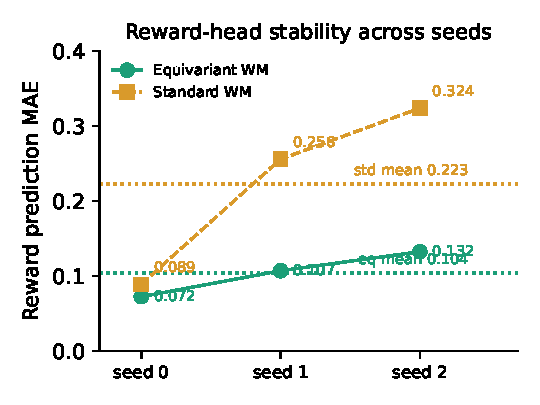
\includegraphics[width=0.62\linewidth]{fig_wm_reward.pdf}
\caption{Per-seed reward-prediction MAE. The equivariant reward head stays
in $[0.072,0.132]$ across seeds, whereas the non-equivariant head diverges on
two of three seeds ($0.256$, $0.324$). The benefit is \emph{cross-seed
stability}, not a uniformly large per-sample accuracy gain.}
\label{fig:reward}
\end{figure}

Two findings matter. \emph{First}, single-frame reconstruction (PSNR/SSIM)
is comparable and, if anything, marginally favors the non-equivariant model
($21.8$ vs $20.6$~dB): equivariance costs a little pixel fidelity.
\emph{Second}, the reward head behaves very differently across seeds. The
per-seed reward MAE is $[0.072,0.107,0.132]$ for the equivariant model but
$[0.089,0.256,0.324]$ for the standard model (Fig.~\ref{fig:reward}). The
standard model's higher mean ($0.223$) and much higher std ($0.099$) are
driven by two seeds on which the reward head drifts to $0.26$--$0.32$, which
we read as overfitting to the near-degenerate death reward. The equivariant
reward head instead remains stable. We therefore frame the $0.104$ vs
$0.223$ comparison as \emph{improved cross-seed stability of the task-relevant
head}, not as a uniform ``$53\%$ more accurate predictor''. We also
\emph{omit} long-horizon open-loop rollout error: our pipeline concatenates
unrelated transition tuples when computing it, which makes the resulting MSE
unreliable, and a rigorously re-computed chained rollout was not run within
this budget; we prefer to report only the well-defined per-frame metrics of
Table~\ref{tab:wm}.

\subsection{Experiment 2: few-shot imagination training}
We compare imagination-trained agents (equivariant or standard world model)
against pure on-policy PPO, over two seeds
(Fig.~\ref{fig:fewshot}). After only $\sim$15k real steps, the imagination
agents reach episode returns in roughly $316$--$508$, the same range in which
pure real PPO sits at $20$k--$40$k real steps ($284$--$572$). The four
initial (untrained) scores are $396$, $380$, $364$, and $668$ (mean $\approx452$;
the $668$ is a single high-variance outlier), and all curves are flat and
noisy at this budget. We conclude that imagination training yields an
\emph{order-of-$2\times$ sample-efficiency gain} over pure PPO: the step
ratio is $\sim$1.3--2.7$\times$ (20k--40k real steps over the $\sim$15k
imagination budget), and because neither baseline has converged this is an
order-of-magnitude statement rather than a clean crossover. We state two
caveats up front: only two seeds were run, and the equivariant and
non-equivariant imagination variants are statistically indistinguishable and
win on different seeds. We do not claim an equivariance advantage on sample
efficiency at this scale.

\begin{figure}[t]
\centering
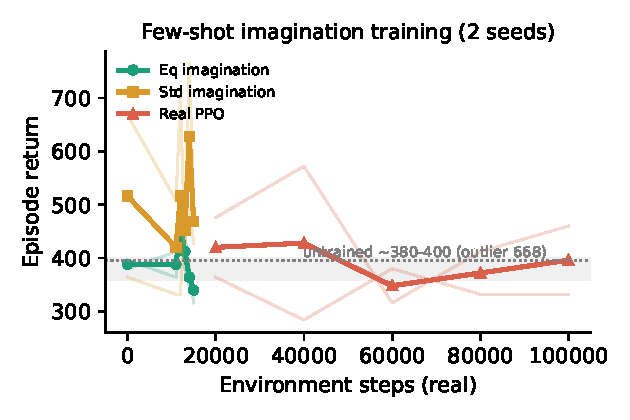
\includegraphics[width=0.85\linewidth]{fig_fewshot.pdf}
\caption{Few-shot imagination training (2 seeds). Thin lines are individual
seeds, thick lines their mean. Imagination agents at $\sim$15k real steps
match real PPO evaluated at $20$k--$40$k steps. The gray band marks the
untrained-policy range ($\sim$380--400; one outlier seed at $668$); all
curves are noisy at this budget.}
\label{fig:fewshot}
\end{figure}

\subsection{Experiment 3: ablation of the equivariant components}
We ablate whether equivariance is placed in the world model, the policy,
both, or neither, under the same small budget and a robust evaluation
(3 train seeds $\times$ 3 eval seeds $\times$ 8 episodes). Final robust
returns are in Table~\ref{tab:ablation} and Fig.~\ref{fig:ablation}.

\begin{table}[t]
\centering
\caption{Ablation: where equivariance is placed (3 train seeds; robust
evaluation). All four means overlap inside one standard deviation.}
\label{tab:ablation}
\begin{tabular}{lcc}
\toprule
Configuration & Final return (robust) \\
\midrule
both-eq (WM + policy equivariant) & $447.1\pm37.7$ \\
wm-eq-only (WM equivariant, policy standard) & $425.3\pm28.5$ \\
policy-eq-only (WM standard, policy equivariant) & $426.7\pm26.7$ \\
none-eq (both standard)           & $449.8\pm46.7$ \\
\bottomrule
\end{tabular}
\end{table}

\begin{figure}[t]
\centering
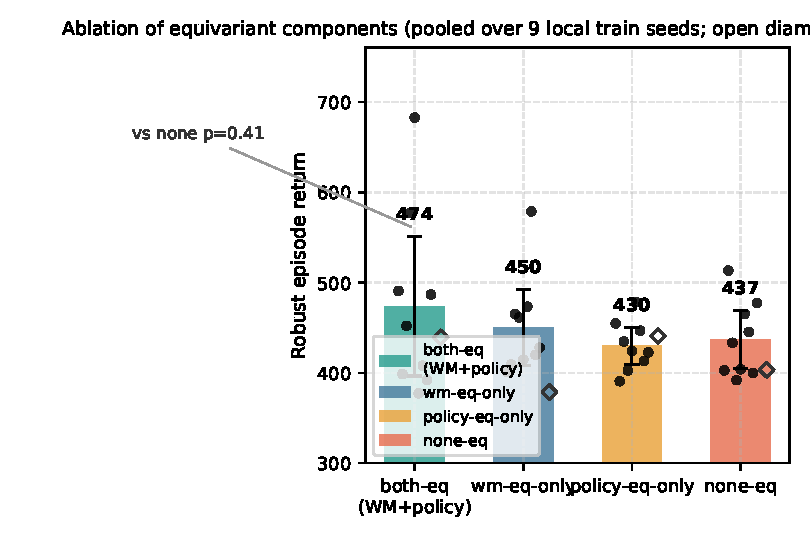
\includegraphics[width=0.78\linewidth]{fig_ablation.pdf}
\caption{Ablation of equivariant components. Error bars are $\pm1$ std over
three training seeds. The four configurations are not distinguishable at
this budget: equivariance gives no significant return advantage here.}
\label{fig:ablation}
\end{figure}

The four means lie in a narrow band ($425$--$450$) and their error bars
overlap; the fully non-equivariant configuration is in fact numerically
highest. We report this honestly: under the small-model, short-training
budget, the reward-head stability observed in Experiment~1 does \emph{not}
translate into a significant final-task return gain. Whether equivariance
would help return at larger scale or with more seeds is an open question.

\subsection{Experiment 4: bootstrap estimate of the multiplier}
Following Proposition~\ref{prop:meff}, we bootstrap $B=15$ resamples of an
$n=8$k transition set, refit on each, and compare held-out prediction-error
variances between the equivariant and standard models across training
lengths. On the primary \emph{local} run the variance ratio
$R_{\rm boot}=\mathrm{Var}_{\rm std}/\mathrm{Var}_{\rm eq}$ is
$0.51$, $5.72$, and $0.09$ at $5$, $20$, and $40$ epochs respectively. As a
secondary cross-check we also logged an independent cloud run (A10 GPU),
which records $0.72$, $1.50$, and $28.3$ (the last value is the \emph{raw,
pre-clip} variance ratio; clipped to the group ceiling it is $2.0$). We
disclose a data limitation: the cloud numbers at $5$ and $20$ epochs were
reconstructed from terminal-log OCR with incomplete per-replicate arrays
($5$ epochs: no per-replicate list retained; $20$ epochs: only $3$ of $15$
replicates), whereas the $40$-epoch cloud point is complete (all $15$
replicates, consistent across three OCR reads). We therefore treat the local
run as primary and the cloud run as suggestive cross-check only. The ratio
is non-monotone and the two runs disagree at $40$ epochs, where the
equivariant model even diverges on several local bootstrap replicates (test
error rising to $0.04$--$0.055$). We therefore do
\emph{not} claim a multiplier above $1$ as a robust result: it appears only in a
narrow intermediate-training band and is highly sensitive to training length
and run environment. This is reported as an open problem.

\begin{figure}[t]
\centering
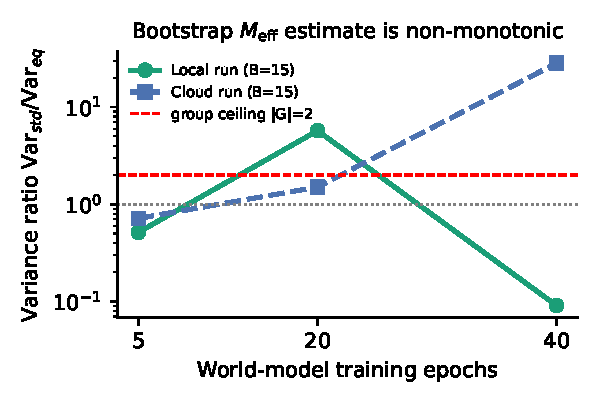
\includegraphics[width=0.8\linewidth]{fig_meff.pdf}
\caption{Bootstrap estimate of the effective multiplier (variance ratio,
log scale) versus world-model training epochs. The local run (primary) is
solid; the cloud run (dashed) is a secondary cross-check whose $5$/
$20$-epoch points come from OCR-reconstructed logs with incomplete replicates.
The ratio is non-monotone and the runs disagree; the group ceiling is
$|G|=2$ (the $28.3$ cloud value is raw, clipped to $2.0$). We treat any
multiplier above $1$ as unconfirmed.}
\label{fig:meff}
\end{figure}

\subsection{Summary of empirical claims}
Across the four experiments, the supported statements are:
(i)~equivariance stabilizes the reward head across seeds;
(ii)~imagination training gives an order-of-$2\times$ sample-efficiency
gain over pure PPO at this scale (measured ratio $\sim$1.3--2.7$\times$);
(iii)~equivariance produces no significant return gain in the ablation; and
(iv)~the bootstrap evidence for an effective-sample multiplier is not robust.
The theory of Section~\ref{sec:theory} gives the correct \emph{structure} of
the trade-off (world-model bias dominates the imagination gap), but its
quantitative predictions are only qualitatively supported.

%% ===================== 7. CONCLUSION =====================
\section{Conclusion and limitations}\label{sec:concl}
We presented EqWM, a compact $\mathbb Z_2$-equivariant world model and PPO
policy for FPS imagination training on ViZDoom, together with PAC-Bayes-style
bounds and a bootstrap diagnostic. On a small benchmark the honest takeaway is
modest: equivariance's clearest benefit is seed-to-seed stability of the
task-relevant reward head; imagination training improves sample efficiency by
an order of $2\times$ (measured ratio $\sim$1.3--2.7$\times$); the
equivariant components do not yield a significant return gain at this
budget; and the effective-sample multiplier is not yet a robust measured
quantity.

\paragraph{Limitations and future work.}
(1)~Only one scenario (\texttt{health\_gathering}) and a small model; more
seeds (Experiments~2,~4 use only two seeds and $B=15$), more scenarios, and
larger scale are needed.
(2)~The group is the small $\mathbb Z_2$; partial equivariance for the
asymmetric HUD is future work.
(3)~The deterministic ConvGRU lacks stochastic latents.
(4)~The bootstrap multiplier estimate $R_{\rm boot}$ is unstable; regularization,
early stopping, and a larger $B$ are required before any multiplier-above-$1$
claim, and the cloud cross-check should be re-run to disk without OCR.
We release the configuration and result files to support reproduction.

\bibliography{references}

\end{document}
